% !TEX program = xelatex
\documentclass[11pt]{article}
\usepackage[margin=1in]{geometry}
\usepackage{nopageno} % no page numbers

\usepackage{graphicx}
\graphicspath{ {./graphics/} }
\usepackage[dvipsnames]{xcolor}
\definecolor{CrispBlue}{HTML}{0176AE}

\usepackage{fontspec}
\usepackage{tcolorbox}
\usepackage{etoolbox}
\BeforeBeginEnvironment{verbatim*}{\begin{tcolorbox}[colback=CrispBlue!5!white,colframe=CrispBlue!75!black]}%
\AfterEndEnvironment{verbatim*}{\end{tcolorbox}}%


\usepackage{hyperref}
\hypersetup{
    colorlinks,
    citecolor=black,
    filecolor=black,
    linkcolor=black,
    urlcolor=black
}

\usepackage{subcaption}
\setlength{\parindent}{0pt}
\setlength{\parskip}{1em}

\usepackage{tocloft}
\renewcommand{\cftpartleader}{\cftdotfill{\cftdotsep}}
\renewcommand{\cftsecleader}{\cftdotfill{\cftdotsep}}

\usepackage{fancyhdr}
\pagestyle{fancy}
\fancyhf{}
\lhead{ECE 517: Machine Learning}
\rhead{Assignment 5}
\rfoot{Page \thepage}

\usepackage{amsmath,amsfonts,amssymb}
\usepackage{bm}
\usepackage{mathtools}

\renewcommand{\listfigurename}{List of Figures}

\begin{document}
\setmainfont{SF Pro Text}
\setsansfont{SF Pro Text}
\setmonofont{SF Mono}
\renewcommand{\familydefault}{\sfdefault}

\thispagestyle{empty}
\begin{titlepage}
\vspace*{\fill}
\begin{center}
\textsc{\Huge{ECE 517: Machine Learning}}\\[3em]
\textsc{\LARGE Assignment 5: Construction of a Regression Algorithm}\\[6em]
\textsc{\Large David Kirby -- 101652098 -- davidkirby@unm.edu}\\[3em]
\textsc{\Large Fall 2021}
\end{center}
\vfill
\begin{figure}[h]
\begin{subfigure}{0.5\textwidth}
\includegraphics[width=0.25\linewidth]{learning.png}
\end{subfigure}
\begin{subfigure}{0.6\textwidth}\hspace{1em}
\includegraphics[width=0.8\linewidth]{new-soe-logo.png}
\end{subfigure}
\end{figure}
\end{titlepage}
\setcounter{figure}{0}

\hypersetup{
    linkcolor=CrispBlue,
    urlcolor=CrispBlue,
    breaklinks=true
}


The .mat and the .csv files provided is a dataset that contains a training and a test sets. Each set consists of the predictor input Xtrain and Xtest for regressors ytrain and ytest, corresponding to the response y of a physical model to a vector signal x of 19 dimensions. The train and test outputs consist of 81 samples and they are depicted in the figure below.

In this assignment, you must construct a linear ridge regression that uses inputs \(X\) to predict \(y\). Use 20\% of the training data to validate gamma. The validation procedure consists of:

\begin{itemize}
    \item Training the predictor with 80\% of the training data and a given value for gamma.
    \item Running a test for the rest of the training data.
    \item Computing the mean square error of the prediction.
    \item Repeat for a reasonable range of gamma.
\end{itemize}

Choose the value of gamma that produced the best result. A reasonable interval can be between 0.01 times and 10 times the trace of the matrix, using a logarithmic spacing. In Matlab, use function logspace.

Provide the following results of the experiment:

\begin{itemize}
    \item A graph comparing the real and predicted data.
    \item A graph of the result ofthevalidation square error.
    \item The value of the optimal validation and test square errors.
\end{itemize}

\begin{tcolorbox}[colback=CrispBlue!5!white,colframe=CrispBlue!75!black,title=Construction of a regression algorithm with the model parameters.]
Using the example regression algorithm provided in the assignment, I swept gamma from 0.1 to 10 times the trace matrix.\vspace{1em}

The optimal value for \(\gamma\) was determined to be 0.004731 which led to an MMSE of 0.00808.

\end{tcolorbox}

\begin{figure}[h!]
    \centering
    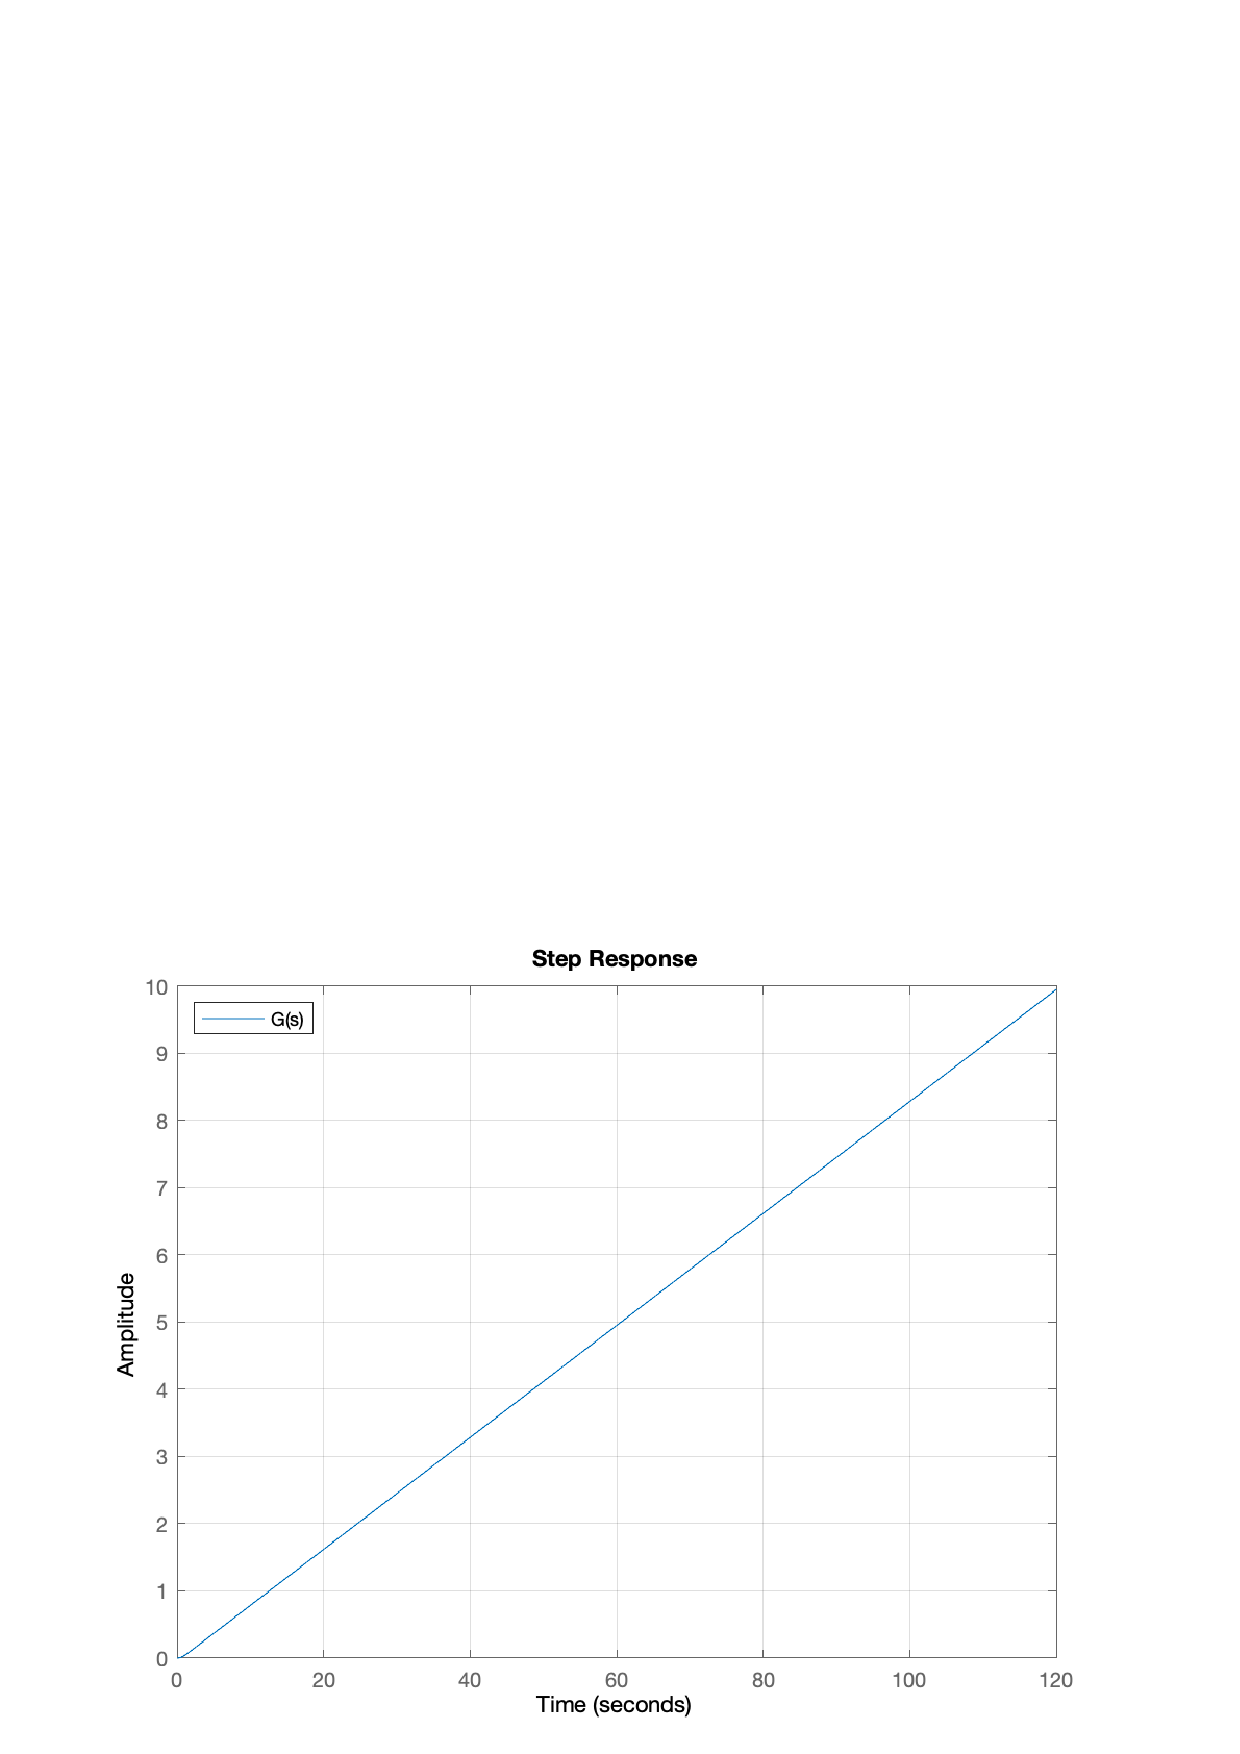
\includegraphics[width=0.8\textwidth]{figure_0.png}
    \vspace{-1em}\caption{Validation mean square error (\(\gamma\) swept from 0.1 to 10).}
    % \label{fig:sampleData}
\end{figure}

\begin{figure}[h!]
    \centering
    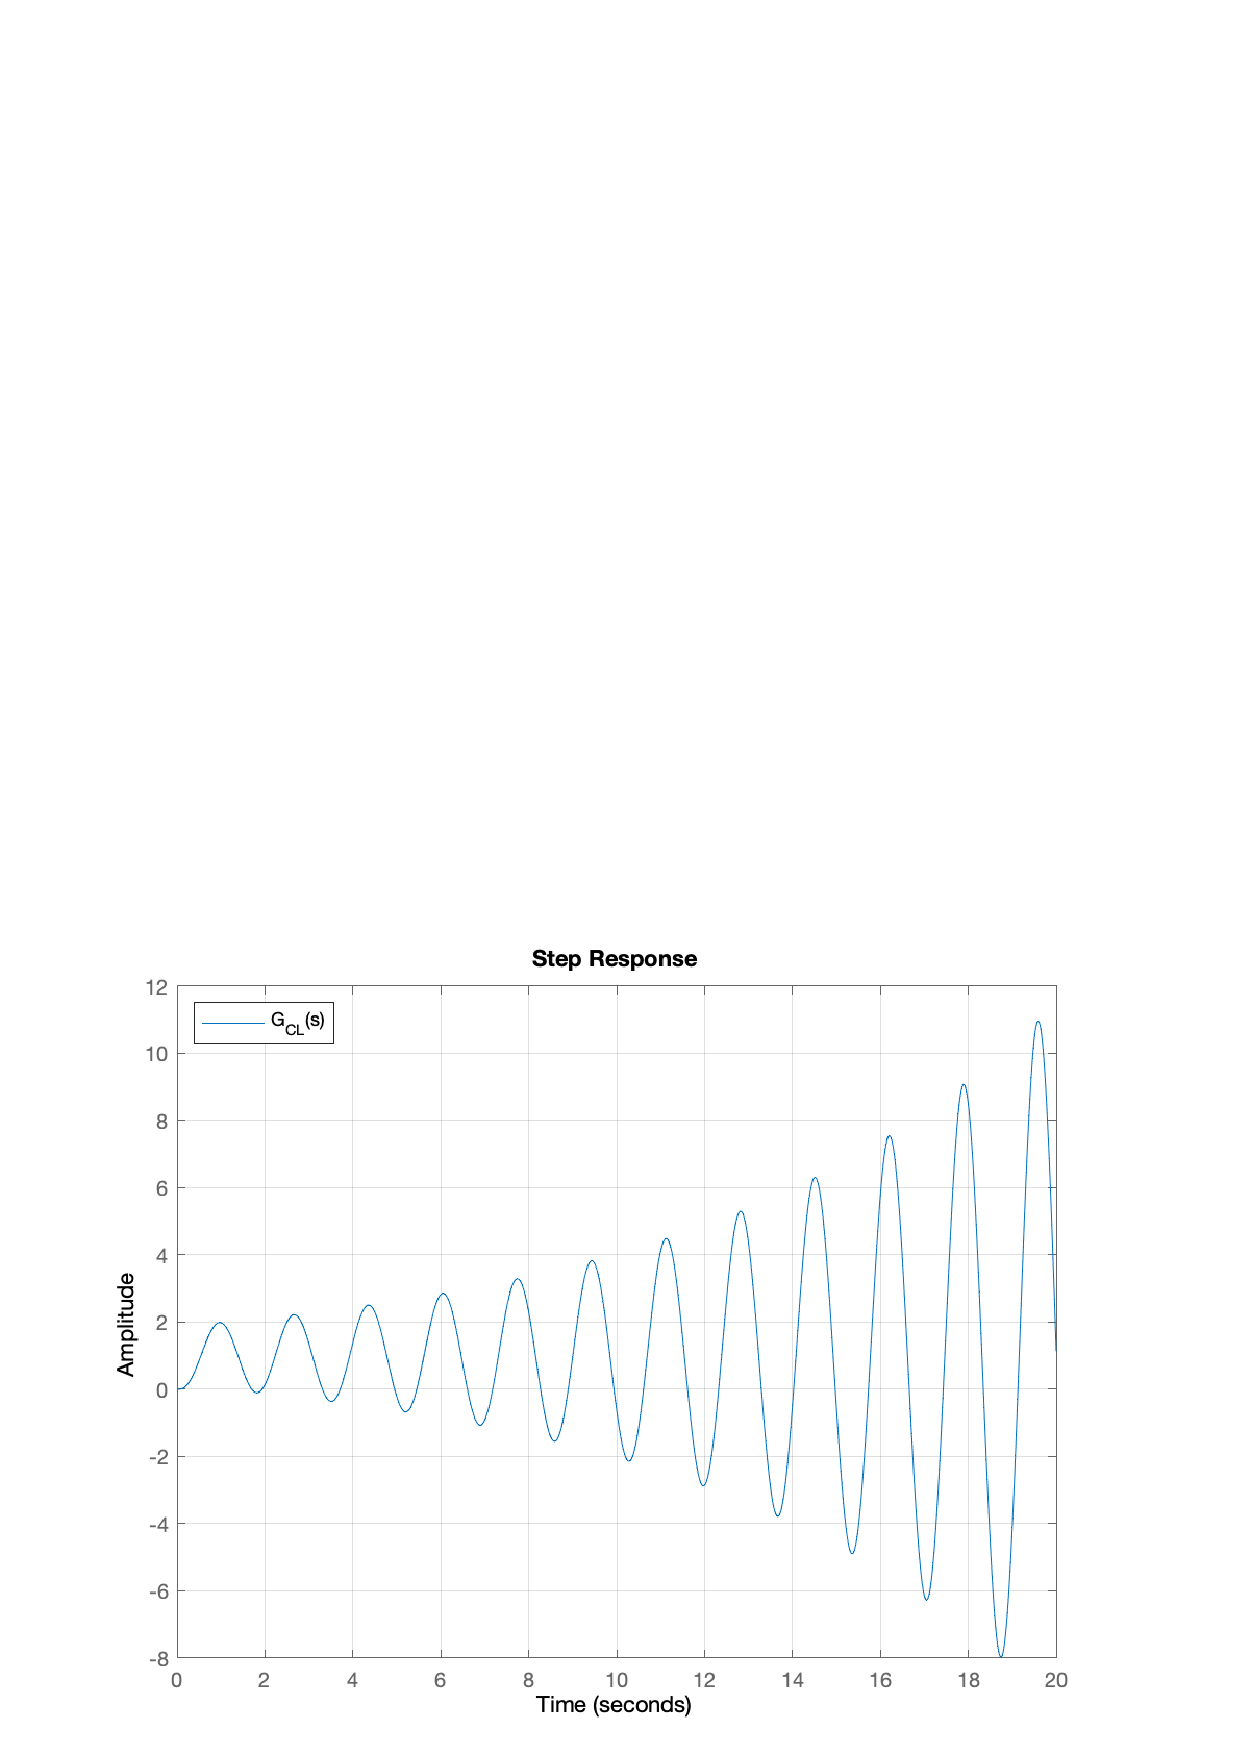
\includegraphics[width=0.8\textwidth]{figure_1.png}
    \vspace{-1em}\caption{Regression test results.}
    % \label{fig:sampleData}
\end{figure}

\newpage
Repeat the experiment above, but using an SVR and a nu-SVR. In both cases you should use a 20\% of the training data in order to validate the parameters of the SVM.

Provide the following results of the experiment:

\begin{itemize}
    \item A graph comparing the real and predicted data.
    \item A graph of the result ofthevalidation square error.
    \item The value of the optimal validation and test square errors.
    \item A written comparison of the results of this experiment and the previous ones.
\end{itemize}

\begin{tcolorbox}[colback=CrispBlue!5!white,colframe=CrispBlue!75!black,title=Repeating the experiment using SVR and nu-SVR.]
    The optimal value for \(\epsilon\) was determined to be 0.01 and \(C = 5\) which led to an MMSE of 0.00576.\vspace{1em}

    The optimal value for \(\nu\) was determined to be 0.4 and \(C = 10\) which led to an MMSE of 0.00557.\vspace{1em}

    All three results are very similar in their results for the MMSE. This makes sense as we are testing all of these algorithms on the same dataset. The reason as to why this might be can be due to the values chosen for the cost and \(\epsilon\) chosen for the SVR machine when creating the classifier/predictor. Similarly, the cost and \(\nu\) values chosen for the nu-SVR machine could also be the reason for the slight difference in accuracy between the machines.
\end{tcolorbox}

\begin{figure}[h!]
    \centering
    \includegraphics[width=0.8\textwidth]{figure_2.png}
    \vspace{-1em}\caption{Validation mean square error (\(\epsilon\)).}
    % \label{fig:sampleData}
\end{figure}

\begin{figure}[h!]
    \centering
    \includegraphics[width=0.8\textwidth]{figure_3.png}
    \vspace{-1em}\caption{SVR test results.}
    % \label{fig:sampleData}
\end{figure}

\begin{figure}[h!]
    \centering
    \includegraphics[width=0.8\textwidth]{figure_4.png}
    \vspace{-1em}\caption{Validation mean square error (\(\nu\)).}
    % \label{fig:sampleData}
\end{figure}

\begin{figure}[h!]
    \centering
    \includegraphics[width=0.8\textwidth]{figure_5.png}
    \vspace{-1em}\caption{nu-SVR test results.}
    % \label{fig:sampleData}
\end{figure}

\end{document}